\documentclass[aspectratio=169]{beamer}

% --------------------
% Sprache & Encoding
% --------------------
\usepackage[ngerman]{babel}
\usepackage[T1]{fontenc}
\usepackage[utf8]{inputenc}

% --------------------
% Design / Theme
% --------------------
\usetheme{CambridgeUS}
\usecolortheme{default}

% --------------------
% Pakete
% --------------------
\usepackage{graphicx}
\usepackage{amsmath}
\usepackage{siunitx}
\usepackage{booktabs}

% --------------------
% Titelinformationen
% --------------------
\title[Kurztitel]{Kick-off Präsentation}
\subtitle{RO45 Robotik Projekt 3 – Automatische Sortieranlage}
\author{NimSort42}
\institute{Hochschule Kempten}
\date{\today}

% Bild für die Titelfolie (Pfad anpassen)
\titlegraphic{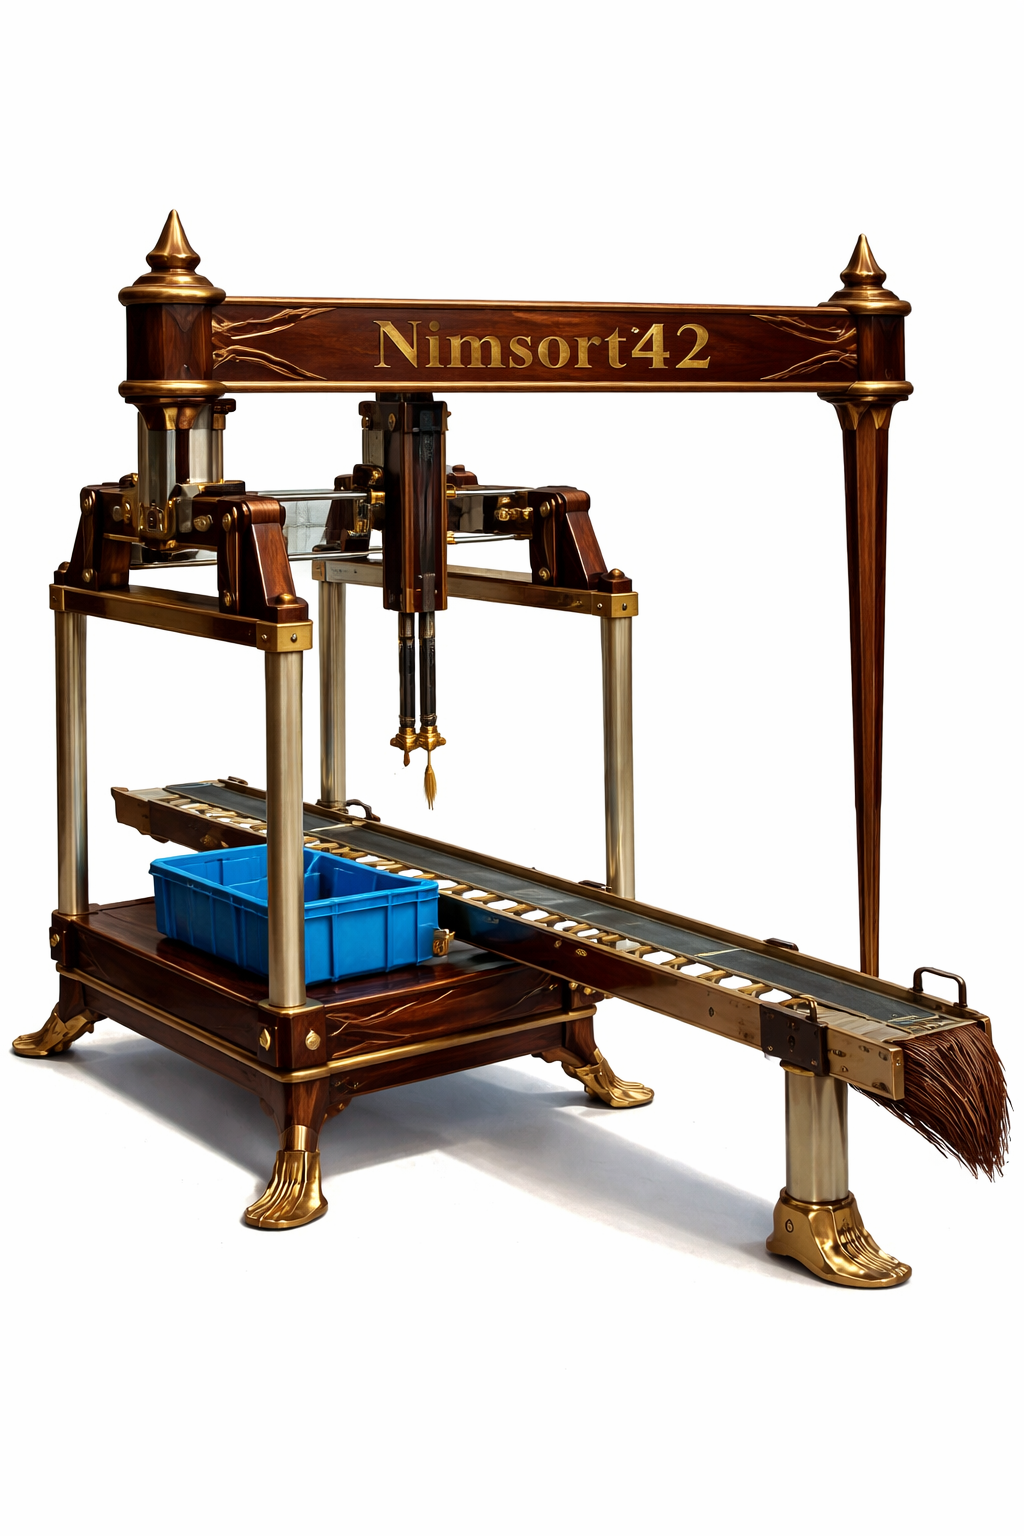
\includegraphics[width=0.135\textwidth]{../pictures/logo_nimsort42.png}}

% TOC Punkte ohne Zahlen
\setbeamertemplate{section in toc}[ball unnumbered]
\setbeamertemplate{subsection in toc}[ball unnumbered]
\setbeamercolor{structure}{fg=black}

% --------------------
% Dokument
% --------------------
\begin{document}
	
	% Titelfolie
	\begin{frame}
		\titlepage
	\end{frame}
	
	% Inhaltsverzeichnis
	\begin{frame}{Inhalt}
		\tableofcontents
	\end{frame}
	
	% --------------------
	\section{Team \& Projekt}
	
	\begin{frame}{Projektteam \& Projektvorstellung}
		\textbf{Projektteam:}
		\begin{itemize}
			\item Bachhuber Yanik
			\item Keppler Benjamin
			\item Moser Louis
		\end{itemize}
		
		\vspace{6mm}
		
		\textbf{Projektvorstellung:}
		\begin{itemize}
			\item Entwicklung einer Software für eine automatische Sortieranlage
			\item Erkennung und Unterscheidung von Katzen und magischen Einhörnern
			\item Zielgerichtetes Aussortieren über einen Portalroboter
			\item Nicht erkannte Objekte werden ignoriert
		\end{itemize}
	\end{frame}
	
	% --------------------
	\section{Projektmanagement}
	
	\begin{frame}{Meilensteine}
		\begin{itemize}
			\item Notwendige Koordinatensysteme festgelegt 1/2
			\item Grundlagen realisieren. 3/4
			\item Prädizierte Positionen im Weltkoordiantensystem Ausgeben 5/6
			\item Regelung auf einen Punkt im Weltkoordinatensystem 7/8
			\item Prozesslogik ist in Python Programmiert und getestet 9
			\item Abschlusspräsentationen 10/11
		\end{itemize}
	\end{frame}
	
	\begin{frame}{Timeline}
		\begin{itemize}
			\item Notwendige Koordinatensysteme festgelegt (16.03) bis (23.03
			\item Kickoff Präsentation mit Softwarearchitektur (24.03) bis (30.03)
			\item Kommunikation mit der Hardware (31.03) bis (06.04)
			\item Vision Basis und Ros Architektur Programmieren (07.04) bis (13.04)
			\item Prädizierte Positionen im Weltkoordiantensystem Ausgeben (14.04) bis (20.04)
			\item Initiale Kalibrierung des Gesamtsystems (21.04) bis (27.04)
			\item Regelung auf einen Punkt im Weltkoordinatensystem (28.04) bis (11.05)
			\item Vision Modell fertigstellen und feinjustieren (12.05) bis (25.05)
			\item Prozesslogik ist in Python Programmiert und getestet (26.05) bis (01.06)
			\item Finaler Test und Doku (16.06) bis (22.06)
			\item Abschlusspräsentationen (23.06) bis (29.06)
		\end{itemize}
	\end{frame}
	
	\begin{frame}{Risikomanagement}
		\textbf{Mögliche Risiken:}
		\begin{itemize}
			\item \begin{tabular}[t]{@{}p{7.5cm} l@{}}
				Hardware steht nicht rechtzeitig zur Verfügung & $\Rightarrow$ Zeitverzug
			\end{tabular}
			\item \begin{tabular}[t]{@{}p{7.5cm} l@{}}
				Ausfall eines Teammitglieds & $\Rightarrow$ Mehrbelastung des Teams
			\end{tabular}
			\item \begin{tabular}[t]{@{}p{7.5cm} l@{}}
				Professor fällt aus & $\Rightarrow$ Projekt kann nicht bewertet werden
			\end{tabular}
			\item \begin{tabular}[t]{@{}p{7.5cm} l@{}}
				Eingeschränkte Hardwareverfügbarkeit & $\Rightarrow$ Weniger Tests
			\end{tabular}
		\end{itemize}
	\end{frame}
	
\begin{frame}{Stakeholder}
	\begin{itemize}
		\item \begin{tabular}[t]{@{}p{3cm} l@{}}
			Teammitglieder & $\Rightarrow$ Bestehen des Moduls
		\end{tabular}
		\item \begin{tabular}[t]{@{}p{3cm} l@{}}
			Professor & $\Rightarrow$ Durchführung und Bewertung des Projekts
		\end{tabular}
		\item \begin{tabular}[t]{@{}p{3cm} l@{}}
			Kunde (Haribo) & $\Rightarrow$ Zuverlässige Sortieranlage
		\end{tabular}
	\end{itemize}
\end{frame}
	
	
	\begin{frame}{Hauptverantwortlichkeiten}
		\begin{tabular}{@{}l l@{}}
			\textbf{Bachhuber Yanik} & $\Rightarrow$ Prozesslogik, Initialisierung \\ 
			\textbf{Keppler Benjamin} & $\Rightarrow$ Regelung, Achsensteuerung \\
			\textbf{Moser Louis} & $\Rightarrow$ Vision Pipeline, Objekterkennung \\
		\end{tabular}
	\end{frame}
	
	% --------------------
	\section{Technische Realisierung}
	
	\begin{frame}{Hardware}
		\begin{itemize}
			\item Portalroboter mit Sauggreifer (Arbeitsraum: $\SI{0.1}{m}^3$)
			\item Förderband mit variabler Geschwindigkeit ($0$–$\SI{0.05}{m/s}$)
			\item Arduino Mega mit Stepper Shield zur Achsansteuerung
			\item ELP USB Kamera (2.0 MP) zur Objekterkennung
			\item Zwei Sortierkisten (Katze / Einhorn) und eine Restkiste
		\end{itemize}
	\end{frame}
	
	\begin{frame}{Software}
		\begin{itemize}
			\item Betriebssystem: Ubuntu 22.04
			\item Framework: ROS2 Humble Hawksbill
			\item Vision-Software zur Objektklassifikation (Machine Learning)
			\item ROS2-Knoten für:
			\begin{itemize}
				\item Kameraverarbeitung und Objekterkennung
				\item Positionsbestimmung im Weltkoordinatensystem
				\item Regelung und Ansteuerung der Achsen
			\end{itemize}
		\end{itemize}
	\end{frame}
	
	\begin{frame}{Architektur}
		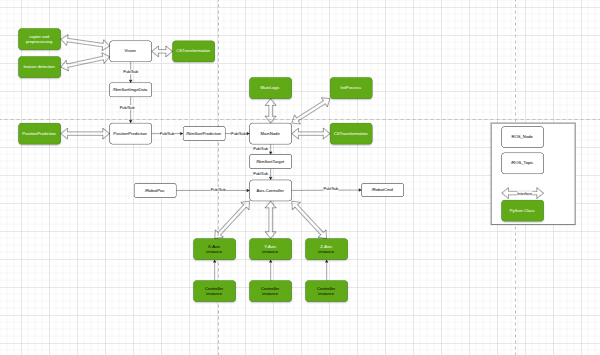
\includegraphics[width=\textwidth]{../pictures/software_architektur.png}
	\end{frame}
	
	% --------------------
	\begin{frame}{Fragen}
		\centering
		\Huge Vielen Dank für Ihre Aufmerksamkeit
	\end{frame}
	
\end{document}